\documentclass[output=paper]{langscibook}
\ChapterDOI{10.5281/zenodo.8124500}
\author{Rafael Orozco\orcid{0000-0001-9232-0287}\affiliation{Louisiana State University} and Luz Marcela Hurtado\orcid{}\affiliation{Central Michigan University} and Marianne Dieck\orcid{}\affiliation{Universidad de Antioquia}}
\title[Toward the prevalence of a personal use of impersonal \textit{uno} in C.S.]
       {Toward the prevalence of a personal use of impersonal \textit{uno} in Colombian Spanish}
\abstract{This variationist study explores the alternation between the pronouns \textit{uno} ‘one’ and \textit{yo} ‘I’ in Colombian Spanish using data from the PRESEEA Medellín corpus. We test the hypothesis that, in Colombian Spanish, \textit{uno} is being recast to the point that it functions as a variant of the first-person singular subject pronoun \textit{yo}. We aim to go beyond the well-established \textit{pronombrista} line of subject pronoun research with a variationist analysis of the alternation between \textit{uno} and \textit{yo} that examines, among other things, the role of stance and the focus of attention in terms of predictors that include transitivity, verb semantics, coreference, type of discourse, and sentence polarity. Our findings uncover the strongest conditioning effect of tense, mood and aspect as well as robust effects of transitivity, discourse genre, polarity, and type of preceding subject. Thus, the \textit{uno/yo} alternation constitutes a linguistic variable in its own right.}
% \smallskip\\
% \textbf{Keywords:} Impersonality, \textit{uno} ‘one’ (subject pronoun), Colombian Spanish, language variation, Medellín, sociolinguistics}


\IfFileExists{../localcommands.tex}{
  \addbibresource{../localbibliography.bib}
  % add all extra packages you need to load to this file

\usepackage{tabularx,multicol}
\usepackage{url}
\urlstyle{same}

\usepackage{listings}
\lstset{basicstyle=\ttfamily,tabsize=2,breaklines=true}

\usepackage{langsci-basic}
\usepackage{langsci-optional}
\usepackage{langsci-lgr}
\usepackage{langsci-osl}
% \usepackage{./langsci/styles/langsci-lgr}
% \usepackage{./langsci/styles/langsci-osl}
% \usepackage{langsci-gb4e}

\usepackage{tikz}
\usetikzlibrary{patterns,calc}
\pgfdeclarepatternformonly{south east lines}{\pgfqpoint{-0pt}{-0pt}}{\pgfqpoint{3pt}{3pt}}{\pgfqpoint{3pt}{3pt}}{
    \pgfsetlinewidth{0.6pt}
    \pgfpathmoveto{\pgfqpoint{0pt}{3pt}}
    \pgfpathlineto{\pgfqpoint{3pt}{0pt}}
    \pgfpathmoveto{\pgfqpoint{.2pt}{-.2pt}}
    \pgfpathlineto{\pgfqpoint{-.2pt}{.2pt}}
    \pgfpathmoveto{\pgfqpoint{3.2pt}{2.8pt}}
    \pgfpathlineto{\pgfqpoint{2.8pt}{3.2pt}}
    \pgfusepath{stroke}}
    
\usepackage{stmaryrd}
\usepackage{wasysym}
\usepackage{multirow}
\usepackage{caption}
\usepackage{subcaption}
\usepackage{mathrsfs}
\usepackage{qtree}

\usepackage{linguex}


  %pminos do not split footnotes
% \interfootnotelinepenalty=10000 %Footnote in Laporte chapters has to be split SN


%\DeclareIndexNameFormat{default}{%
%\nameparts{#1}%
%\usebibmacro{index:name}%
%{\index[names]}%
%{\namepartfamily}%
%{\namepartgiveni}%
% {}% L1
% {}% L2
%{\namepartprefix}% generates spurious space L3
%{\namepartsuffix}% generates spurious space L4
%}

%  {\DeclareIndexNameFormat{default}{%
%     \usebibmacro{index:name}{\index[names]}{#1}{#3}{#5}{#7}}}

%\DeclareIndexNameFormat{default}{%
%  \usebibmacro{index:name}{\sindex[nom]}{#1}{#3}{#5}{#7}}

%\DeclareIndexNameFormat{default}{%
%  \usebibmacro{index:name}{\sindex[person]}{#1}{#3}{#5}{#7}}
%\DeclareIndexNameFormat{default}{%
%\nameparts{#1} \usebibmacro{index:name}{\sindex[person]]}{\namepartfamily}{‌​\namepartgiven}{\nam‌​epartprefix}{\namepa‌​rtsuffix}}

%\newcommand{\smiley}{:)}

%\renewbibmacro*{index:name}[5]{%
%\usebibmacro{index:entry}{#1}%
%{\iffieldundef{usera}{}{\thefield{usera}\actualoperator}\mkbibindexname{#2}{#3}{#4}{#5}}}

% \newcommand{\noop}[1]{}

%remove for final
%\overfullrule=1mm

\newcommand{\tobi}[2]}}
\renewcommand{\S}[1]{\tobi{#1}{\textsc{*}}}

% this volume references
% puts: [this volume]
% already defined: \citetv
%\newcommand{\citepv}[1]{(\citeauthor{#1} \citeyear*{#1} [this volume])}
\newcommand{\citealtv}[1]{\citeauthor{#1} \citeyear*{#1} [this volume]}

%parentheses around example number
\newcommand{\pref}[1]{(\ref{#1})}

% in-text examples

\newcommand{\lnex}[1]{\textit{#1}} %target lang word
\newcommand{\lnlit}[1]{(lit.: `#1')} %literal reading
\newcommand{\lnlat}[1]{(#1)} % latinization
\newcommand{\lntrans}[1]{`#1'} %translation
\newcommand{\lnexl}[2]%
{\lnex{#1}{} \lnlat{#2}} % ex with latinization
\newcommand{\lnexlat}[3]{\lnex{#1}{} \lnlat{#2}{} \lntrans{#3}} % ex with latinization and tranl.

%ch01
\newcommand{\co}[1]{\mbox{\textbf{#1}}}

%ch09

\newcommand{\cyrbulg}[1]{\begin{otherlanguage*}{bulgarian}#1\end{otherlanguage*}}


%ch10
\newcommand{\nlp}{{\small NLP}}
\newcommand{\mwe}{{\small MWE}}
\newcommand{\rae}{{\small RAE}}
\newcommand{\lvc}{{\small LVC}}
\newcommand{\pos}{{\small P}o{\small S}}
%\newcommand{\todo}[1]{ \textcolor{red}{#1} }

%\renewcommand{\labelenumi}{\theenumi}
%\ainamefmt{{vv}{ll}{, ff}{, jj}} % fullname

\newcommand{\biberror}[1]{{\color{red}#1}}

\newcommand{\osenovaitem}{--~} 
  %% hyphenation points for line breaks
%% Normally, automatic hyphenation in LaTeX is very good
%% If a word is mis-hyphenated, add it to this file
%%
%% add information to TeX file before \begin{document} with:
%% %% hyphenation points for line breaks
%% Normally, automatic hyphenation in LaTeX is very good
%% If a word is mis-hyphenated, add it to this file
%%
%% add information to TeX file before \begin{document} with:
%% %% hyphenation points for line breaks
%% Normally, automatic hyphenation in LaTeX is very good
%% If a word is mis-hyphenated, add it to this file
%%
%% add information to TeX file before \begin{document} with:
%% \include{localhyphenation}
\hyphenation{
    Beck-man
    Ngu-yen
    back-chan-nel
    back-chan-nels
    mo-not-o-nous
    ste-reo-typ-i-cal
}

\hyphenation{
    Beck-man
    Ngu-yen
    back-chan-nel
    back-chan-nels
    mo-not-o-nous
    ste-reo-typ-i-cal
}

\hyphenation{
    Beck-man
    Ngu-yen
    back-chan-nel
    back-chan-nels
    mo-not-o-nous
    ste-reo-typ-i-cal
}
 
  \togglepaper[8]%%chapternumber
}{}

\begin{document}
\maketitle 



\section{Introduction} 


\textit{Uno} ‘one’ is a multifunctional Spanish subject pronoun with third person singular morphosyntax whose pragmatic domain extends to other grammatical persons, mainly the first. \textit{Uno} has traditionally been associated with the expression of impersonality because its association with the first person – both singular and plural – involves connotations of genericity. Studies on impersonality employing semantic, syntactic, and pragmatic approaches have shown that impersonals are versatile with respect to their referential interpretation \parencites[376]{CasiellesSuárez1996}[160]{Hernanz1990}[]{HurtadoGutiérrez-Rivas2016}. Their versatility is such that impersonals can coincide and fulfill the tripartite function of (1) hiding an agent or reducing the speaker’s prominence (\citealt{Barrajón2005, GómezTorrego1992, Haverkate1987, Hernanz1990, HollaenderJensen2002, MuñizCachón1998, RicosVidal2002}); (2) integrating the speaker, involving the interlocutor, and alluding to a group (\citealt{Fernández2008, FernándezRamírez1986, Gelabert-Desnoyer2008, MuñizCachón1998}); and (3) denoting all speakers; i.e., humankind  (\citealt{CompanyPozas2009, FernándezSoriano1999, Siewierska2008}). That is, impersonals display different degrees of specificity and inclusion of the agent. However, some scholars such as \citet[1206]{CompanyPozas2009} also raise the possibility of the complete reduction of the impersonal reference when textual elements such as first-person singular subjects appear; that is, a more personal reading as in the case of example \REF{ex:orozco:1}, from of our dataset.\footnote{Throughout this chapter, we have indicated null subjects using [∅] in the Spanish examples. In the corresponding English translations, null subjects are indicated within backets as well.}



\eanoraggedright\label{ex:orozco:1}
\begin{otherlanguage}{spanish}
eh si es un día laboral /  pues \ExHighlight{uno} \ExHighlight{se} \ExHighlight{levanta} /  obviamente \ExHighlight{[∅]} \ExHighlight{se} \ExHighlight{baña} /  \ExHighlight{[∅]} \ExHighlight{se} \ExHighlight{va} para el trabajo /  ah no /  \ExHighlight{[∅]} \ExHighlight{despacha} a los hijos /  \ExHighlight{[∅]} \ExHighlight{llevo} la señora al trabajo /  al trabajo de ella obviamente /  y \ExHighlight{[∅]} \ExHighlight{me} \ExHighlight{voy} ya para el trabajo mío y \ExHighlight{[∅]} \ExHighlight{ya} \ExHighlight{regreso} después de las seis de la tarde.  (MEDE\_H12\_3)
\end{otherlanguage}
\glt ‘eh if it’s a weekday /  well \ExHighlight{one}\footnote{In most cases, Spanish \ExHighlight{\textit{uno}} would translate as (impersonal) \ExHighlight{you} in colloquial contemporary English. However, given that our paper deals with the \textit{uno/yo} alternation in Spanish, we have translated \ExHighlight{\textit{uno}} as (the less commonly used English equivalent) \ExHighlight{one}.} \ExHighlight{gets} \ExHighlight{up} /  obviously [\ExHighlight{one}] \ExHighlight{bathes} /  [\ExHighlight{one}] \ExHighlight{goes} to work /  ah no /  [\ExHighlight{one}] \ExHighlight{sends} the children off /  [\ExHighlight{I}] \ExHighlight{take} my wife to work /  to her work obviously /  and [\ExHighlight{I}] \ExHighlight{go} to work and [\ExHighlight{I}] \ExHighlight{return} after six in the evening.’  
\z 


In \REF{ex:orozco:1} we observe that the use of \textit{uno} ‘one’ allows a definite reading in connection with the first person and the speaker’s perspective \citep[19]{Haverkate1985}, depending on the contextual cues \citep{Gelabert-Desnoyer2008}. 



This variationist study goes beyond the traditional analysis of the alternation between null and overt subjects in Spanish addressed in the vast \textit{pronombrista} or \textit{pronombrismo} literature (cf. \citealt{CarvalhoShin2015, OrozcoHurtado2021, OtheguyZentella2012}; inter alia), i.e., the research strand devoted to the study of subject pronoun expression (SPE). We explore the variable alternation between the subject pronouns \textit{uno} ‘one’ and \textit{yo} ‘I’ in the Spanish of Medellín, Colombia. Our study is motivated by recent findings from Colombian Spanish (\citealt{Hurtado2015, HurtadoGutiérrez-Rivas2016, HurtadoOrtega-Santos2019, OrozcoHurtado2021,OrozcoHurtado2021b}) that report the impersonal pronoun \textit{uno} being used primarily with referential interpretation in which the connection with the I-speaker as a marker of positioning and subjectivation of discourse prevails.



Given that the interpretation of \textit{uno} as an alternate to \textit{yo} predominates within the range of referential interpretations of \textit{uno,} in the present investigation, we seek to explore whether this role constitutes an indication that \textit{uno} behaves in a more definite and personal way in Colombian Spanish. As our findings will show, the \textit{uno/yo} alternation constitutes a linguistic variable in its own right with its own internal conditioning. The remainder of this chapter is organized as follows: We discuss impersonality and the nature of \textit{uno} in the next section. \sectref{sec:orozco:3} is devoted to the methodological approach, including descriptions of the speech community, the corpus, the dataset, the envelope of variation, our research questions and hypothesis. \sectref{sec:orozco:4} is dedicated to the presentation of our results. \sectref{sec:orozco:5} and \sectref{sec:orozco:6} respectively present the discussion of findings and the conclusion.  



\section{Background}\label{sec:orozco:2}


The frequent occurrence of \textit{uno} with first person singular interpretation has been attested in studies that integrate semantic-pragmatic and social predictors. For instance, \citet{Morales1995} finds that Spanish/English bilingual speakers favor impersonal \textit{tú} ‘you’ and \textit{uno} ‘one’ in the narration of personal experiences. \citet{Fernández2008} points out the influence of the type of information that is transmitted and the speaker’s access to the source of information. According to this scholar, speakers generalize by using \textit{uno} and \textit{tú} departing from the perspective of their own experience and by using the clitic \textit{se} to include other generally accepted voices or opinions. \citet{BassaVanrell2013} also indicates that the predominant referential interpretation for \textit{uno} in Puerto Rico and the Dominican Republic is linked to the speaker’s situation. Additionally, with regard to the social conditioning, \citet{Guirado2011},  \citet{RodríguezAlfano2004}, and \citet{GuantivaAcosta2000} correlate the use of \textit{uno} with the lower socioeconomic levels in Caracas, Monterrey, and Bogotá, respectively. 



Impersonality in Colombian Spanish has been explored in the varieties spoken in the Andean and Caribbean regions as well as among diasporic speakers residing in the United States. These studies have uncovered that \textit{uno} is the predominant form of impersonalization, as follows. In the Andean varieties, \textit{uno} with a frequency of 51\% and \textit{se} with 43.5\% are the most frequent in Bogotá \citep[184]{Hurtado2016}. In Medellín, \textit{uno} with a frequency of 47.9\% and \textit{se} with 27.5\% are the most used impersonals \citep[160]{Dieck2016}. In the Caribbean city of Barranquilla, the use of \textit{uno} prevails with a frequency of 61.6\%, followed by \textit{se} with 25.1\% (\citealt{HurtadoGutiérrez-Rivas2016}: 45). Moreover, in Westchester county and Albany, NY, U.S., among bilingual speakers originally from Bogotá, Valle del Cauca, Antioquia, and Quindío \textit{uno} registers a frequency of 62.6\% followed by \textit{se} with 25.5\%, and impersonal \textit{tú} ‘you’ with 11.9\% \citep[152]{Ramírez2007}.    



The predominant use of \textit{uno} with direct reference to the speaker’s situation – i.e., first person singular interpretation – has been analyzed as a positioning and subjectivization of discourse strategy (\citealt{Hurtado2015}, \citealt{HurtadoGutiérrez-Rivas2016}, \citealt{Ramírez2007}). The referential interpretation of \textit{uno} as a substitute for \textit{yo} – referring only to the speaker – dominates in Bogotá (87\%, weight 0.85) together with a high overt pronominal rate (83\%). This dominance of \textit{uno} reported by \citet{Hurtado2015} appears to increase the attention to the subject’s referent. Likewise, \textit{uno} occurs mainly with verbs whose lexical content indicates feelings, states, and opinions; that is, verbs linked to the speaker’s subjectivity \citep[136-137]{Hurtado2015}. In Barranquilla, \textit{uno} predominantly functions as a variant of \textit{yo} (89.3\%, weight 0.73). Moreover, \textit{uno} appears to denote positioning by being used mainly with verbs that indicate the speaker’s knowledge, evaluation, feelings, and location (\citealt{HurtadoGutiérrez-Rivas2016}: 56). These studies indicate that semantic constraints such as the verb’s referential interpretation and semantic class condition the use of \textit{uno} in Barranquilla and Bogotá.  



Notwithstanding, the variable alternation between \textit{uno} and \textit{yo} remains unexplored in variationist sociolinguistics. Among the few existing investigations, \citet{Flores-Ferrán2009} analyzes this phenomenon among speakers of Colombian, Cuban, Dominican, Mexican, Puerto Rican, and Uruguayan Spanish residing in metropolitan New York City. She finds that the use of \textit{uno} is conditioned by several predictors including semantic clause type, semantic verb type, discourse type, and speaker’s age. Thus, the current investigation addresses the dearth of research on the \textit{uno/yo} alternation and is motivated by recent findings on subject pronoun expression in Barranquilla and Medellín. \citet{HurtadoOrtega-Santos2019} show the effect of high transitivity verbs and the focus of attention on the object in disfavoring the use of overt \textit{uno} in Barranquilla (probability weight of 0.47 for monotransitives and 0.37 for ditransitives). They provide evidence that when the number of participants increases, the competition for the focus of attention also increases, which disfavors the use of overt subject pronouns (previously suggested by \citealt{AijónOlivaSerrano2013} and \citealt{Posio2011}). This result suggests its potential influence on the \textit{uno/yo} alternation.  \citet[14]{OrozcoHurtado2021} report that third person singular pronouns favor overt subjects in Medellín (probability weight 0.64, 42\%). A subsequent analysis (\citealt{HurtadoOrozco2022}), separating \textit{uno} from the other third person singular pronouns (\textit{ella} ‘she’ and \textit{él} ‘he’), reveals that the favorable effect of third person pronouns on overt subjects is driven by \textit{uno} (weight 0.83, 60\%) whereas the other third person singular pronouns have a neutral effect (0.49). Thus, \textit{uno} registers the highest overt pronominal rate in Medellín (60\%) while the other third person singular pronouns \textit{ella} and \textit{él} combined have a modest pronominal rate of 27\%.  



\section{Methodology\label{sec:orozco:3}}


This section describes the speech community constituted by the city of Medellín, the corpus, and the dataset analyzed. It also presents the research questions and hypothesis that guide this investigation, and describes the predictors explored as well as the envelope of variation. 




\subsection{The speech community and the dataset}\label{sec:orozco:3.1}


Medellín, founded in 1675, has constituted one of Colombia’s main industrial centers since the early 20th Century. Between 1890 and 1950, the process of textile industrialization and the production of beer, ceramics, glass, tobacco, and coffee promoted an increment of the blue-collar population as well as the urbanistic growth of the city \citep[8-10]{Botero1996}. According to the 2018 census, Medellín has a population of 2,372,330 out of which 59\% were born in the city, 37\% were born elsewhere in Colombia, and 2.2\% abroad. This reflects the migration and displacement to urban centers Colombians suffered in the latter years of the 20\textsuperscript{th} century because of social unrest and lack of economic opportunities \parencites[]{DepartamentoAdministrativoNacionaldeEstadísticaDANE2019}[82]{Castañeda2005}. 



Medellín Spanish belongs to what  \citet{MontesGiraldo1982} classified as Western Andean Colombian Spanish. The city is located in the department of Antioquia, where two dialectal varieties, the Andean and the Caribbean converge. Because of its geographical location, Medellín developed as an isolated city with differentiated traditions, religious orientation, and family values (\citealt{FernándezAcosta2020}: 95). The Spanish of this region is characterized by the extensive use of the second person singular pronoun \textit{vos} ‘you’ across ages, socioeconomic levels, and registers, which has been analyzed not only as an indicator of an egalitarian and open society (\citealt{MontesGiraldo1967}: 25), but as an expression of local identity and belonging to the region (\citealt{FernándezAcosta2020}: 97). 



Our dataset was culled from the \textit{Proyecto para el Estudio Sociolingüístico del Español de España y de América (PRESEEA) Medellín Corpus} collected between 2007 and 2010 \citep{González-Rátiva2008}. The PRESEEA Medellín corpus interviews contain important cultural and sociolinguistic information about the people, customs, and life in the city. They were carried out using topics prepared to elicit conversation. The predominant form of address used by interviewers was \textit{usted} (formal ‘you’). Questions deal with a variety of topics, from weather, the neighborhood, Medellín’s people, problems in the city, and transportation, to more personal topics including family, work, daily routines, traditions, and holidays. The interviews ended with narrations of a dream or a scary event. We used a subset of 40 of the 119 socially stratified interviews in the corpus, which correspond to 20 women and 20 men whose ages ranged from 15 to 85 years old at data collection time (See \tabref{tab:orozco:1}). All consultants were born in Medellín or in the surrounding region. 


\begin{table}
\begin{tabular}{lcccc}
\lsptoprule
       & \multicolumn{3}{c}{Socioeconomic level} & \\\cmidrule(lr){2-4}
Gender & Low & Mid & Mid-High & Total\\
\midrule
 Women &  8 &  6 &  6 & 20\\
 Men &  8 &  6 &  6 &  20\\
\midrule
Total & 16 & 12 & 12 & 40\\
\lspbottomrule
\end{tabular}
\caption{The speakers.\label{tab:orozco:1}}
\end{table}


\subsection{Research questions and hypothesis}\label{sec:orozco:3.2}


The present investigation is guided by the following research questions and a main hypothesis. We seek to answer three main research questions. 


\begin{enumerate}
  \item How are \textit{uno} and \textit{yo} distributed when they appear interchangeably within a single speech turn, and what predictor variables condition their alternation? 
  \item In what discursive contexts are \textit{uno} and \textit{yo} used interchangeably? 
  \item What functions are most commonly assumed by each pronoun, and how do \textit{uno} and \textit{yo} construct/create the discursive subject?  
\end{enumerate}


Concurrently, we aim to probe the following main hypothesis: \textit{The predominance of} uno \textit{as a substitute of} yo\textit{, within the range of referential interpretations, constitutes an indication that} uno \textit{behaves particularly in a more definite and personal way in Colombian Spanish}. Our hypothesis and research questions were informed by recent investigations of subject pronoun expression and impersonality in Colombian Spanish (\citealt{Dieck2016, Hurtado2015, HurtadoGutiérrez-Rivas2016, HurtadoOrtega-Santos2019, Olave-AriasEtAl2021, Orozco2018, OrozcoHurtado2021}).




\subsection{Predictor variables explored}\label{sec:orozco:3.3}



To answer the above research questions and probe our main hypothesis, we explore the effects of six predictor variables which provide information about the focus of attention and stance. These predictors operate at different morphosyntactic and discourse levels. They can be divided into two main categories:  

\begin{itemize}
    \item Predictors related to the whole clause: \textit{discourse genre, type of preceding subject, polarity,} and \textit{attenuation procedure and genericity inducers}, and 
    \item Predictors related to the verb phrase: \textit{transitivity} and \textit{verb tense, mood and aspect [TMA]}. 
\end{itemize}

As with our research questions and hypothesis, our choice of these predictor variables was guided by the findings of relevant investigations of the expression of impersonality (\citealt{DeCock2014, Flores-Ferrán2009, Guirado2011, GonzálezVergaraRojas2012, Hernanz1990, HurtadoOrtega-Santos2019, OrozcoHurtado2021b, RepedeLeon-Castro2019}). 



To analyze the role of the focus of attention, we considered the relationship between the predictors analyzed and some of Hopper \& Thompson’s transitivity components (\citeyear[252]{HopperThompson1980}). As done by \citet{AijónOlivaSerrano2013}, \citet{HurtadoOrtega-Santos2019}, and \citet{Posio2011}, we probe the premise that transitivity relates to the subject referent’s focus of attention. We also test the notion that high transitivity components (e.g., perfective aspect, realis mode, two or more participants, and affirmative clauses) increase the possibility that attention focuses on the action expressed by the verb and on the object’s reference.   


\subsubsection{Clause-related predictors}\label{sec:orozco:3.3.1}

\subsubsubsection{Discourse genre}\label{sec:orozco:3.3.1.1}
 
We explore the effect of discourse genre seeking to provide a detailed analysis of the role of the speaker’s stance, understood as the manifestation of attitudes, feelings, judgment or commitment to their speech (\citealt{BiberFinegan1988}). In so doing, we analyzed the impact of various discursive modes to measure the effect of realis and irrealis events – one of \citegen{HopperThompson1980} transitivity components – on the \textit{uno/yo} alternation in terms of the following three factors: 

\begin{description}
   \item[Narrative:] personal experiences, daily routine, events that happened in the past or are currently happening (as in example \ref{ex:orozco:1}), 
   \item[Opinion:] argumentative discourse about the city and its people (example \ref{ex:orozco:2}), and 
   \item[Hypothetical situations:] projected and contrary to fact actions (example \ref{ex:orozco:3}). 
\end{description}


\citet[53]{HurtadoOrtega-Santos2019} found a predominant use of \textit{uno} in Barranquilla, Colombia, with factual events, according to the following distribution: narration of personal experiences (80\%), general facts (13\%) and hypotheses and conjectures (7\%). Thus, we seek to determine whether a) this trend extends to contexts in which \textit{uno} and \textit{yo} alternate, or b) the use of \textit{uno} predominates with more irrealis types of discourse (hypothetical situations, opinions) – commonly associated with generalizations or impersonal interpretations – whereas \textit{yo} predominates with more subjective discourse (personal experience narratives), as illustrated in \REF{ex:orozco:2} and \REF{ex:orozco:3}.


\eanoraggedright\label{ex:orozco:2}
\ExHighlight{Yo soy} partidario de eso / \ExHighlight{yo creo} en eso / que a veces la suerte influye en muchas cosas / aunque no \ExHighlight{debe depender uno} / eeh / completamente de eso. (MEDE\_H23\_5) 
\glt ‘\ExHighlight{I’m} a supporter of that / \ExHighlight{I} \ExHighlight{believe} in that / that sometimes luck influences many things / although \ExHighlight{one} \ExHighlight{shouldn't} \ExHighlight{depend} / eeh / completely on that.’
\ex\label{ex:orozco:3}
\begin{xlist}
\exi{E:} ¿cómo cree que sería vivir en otro barrio?
\glt ‘What do you think it would be like to live in another neighborhood?’

\exi {I:}  pues / la verdad \ExHighlight{[${\emptyset}$] no sé} / porque nunca \ExHighlight{[${\emptyset}$] he vivido} en otro barrio / pero \ExHighlight{yo} \ExHighlight{digo} que eso depende como la zona en la que \ExHighlight{uno} \ExHighlight{viva} / depende de los vecinos / como de la interacción que \ExHighlight{uno} \ExHighlight{tenga} con ellos.\\(\ExHighlight{{MEDE\_M03\_5)}}
\glt ‘well / the truth \ExHighlight{{[I]} \ExHighlight{don't} \ExHighlight{know}} / because \ExHighlight{{[I]'ve} \ExHighlight{never} \ExHighlight{lived}} in another neighborhood / but \ExHighlight{{I} \ExHighlight{say}} that it depends on the area where \ExHighlight{{one} \ExHighlight{lives}} / it depends on your neighbors / like on the interaction \ExHighlight{{one} \ExHighlight{has}} with them.’
\end{xlist}
\z 


\subsubsubsection{Type of preceding subject}\label{sec:orozco:3.3.1.2}


This predictor variable explores the possibility that an immediately preceding overt or null subject triggers the occurrence of either \textit{uno} or \textit{yo}. The type of preceding subject predictor relates to priming, a construct based on the premise that speech is cognitively patterned according to preceding discourse \citep{Travis2007}. Though priming was earlier considered to be of linguistic nature, it has been reclassified as a cognitive constraint (cf. \citealt{Labov2010}, \citealt{TammingaEmbick2016}). In \textit{pronombrista} studies, priming explores the possibility that the occurrence of a prior overt or null subject triggers further pronoun expression or omission (\citealt{CameronFlores-Ferrán2004}). Studies on Colombian Spanish (\citealt{TorresCacoullosTravis2019, Travis2005, Travis2007}), Peninsular and Puerto Rican Spanish (\citealt{Cameron1994, Flores-Ferrán2002}) have found significant priming effects on SPE and its intersections with coreference, distance from the preceding coreferential subject, and type of discourse. 



Priming is illustrated in \REF{ex:orozco:4} where the first overt pronominal subject (\textbf{\textit{uno}} \textit{cogía} ‘\textbf{one} would take’) triggers three successive overt \textbf{\textit{uno}} pronominal subjects. Then, the null pronominal subject in [\EmphEmptySet{∅}] \textit{tiene} ‘[\textbf{one}] has’ triggers another null subject in [\EmphEmptySet{∅}] \textit{he visto} ‘[\textbf{I}] have seen.’  



\eanoraggedright\label{ex:orozco:4}
{… en ese entonces} \ExHighlight{{uno} \ExHighlight{cogía}} {de un barrio al centro un bus // me recuerda mucho eso porque cuando} \ExHighlight{{uno} \ExHighlight{llegaba}} {a / a la / al río Medellín // habían unos puentes // que eran como muy inclinados / entonces el bus subía y cuando bajaba //} \ExHighlight{{uno} \ExHighlight{sentía}} {un vacío muy profundo // entonces eso le causaba a uno como susto / como miedo // y en cambio ahora ya los puentes son como diferentes / ya} \ExHighlight{{uno} \ExHighlight{no} \ExHighlight{siente}} {pues esos vacíos //} \ExHighlight{{[∅]} \ExHighlight{tiene}} {como mejor / están mejor diseñados // y pues muy cambiado / y hay espacios también peatonales que no había // eeh lo que sí} \ExHighlight{{[∅]} \ExHighlight{he} \ExHighlight{visto}} {mucho es que / ha habido mucho aumento de carros / de motos de // de vehículos…} (MEDE H21-2)
\glt ‘… in those days \ExHighlight{one} \ExHighlight{would} \ExHighlight{take} a bus from a neighborhood to the city center / I remember that a lot because when \ExHighlight{one} \ExHighlight{arrived} at / at  the / at the Medellín River // there were some bridges // that were like very steep / then the bus would go up and when it went down // \ExHighlight{one} \ExHighlight{felt} a very deep vacuum // then that would give you like a fright / like fear // and instead now the bridges are like different / \ExHighlight{one} no longer \ExHighlight{feels} well those gaps // [\ExHighlight{one}] \ExHighlight{has} like better / [they] are better designed // and well very changed / and there are pedestrian spaces too that didn’t exist // eeh what [\ExHighlight{I}] \ExHighlight{have} \ExHighlight{seen} a lot is that / there has been a great increase in cars / in motorcycles of // in vehicles…’
\z 

Given that priming is a robust SPE predictor in Medellín, we aim to explore its effect on the alternation between \textit{uno} and \textit{yo} in that speech community. Guided by prior \textit{pronombrista} research \citep{Orozco2018}, we tested the effect of perseverance using three factors to code our tokens according to their preceding subject as follows: 1) pronominal overt subject, 2) null subject, and 3) other subjects. The latter factor includes lexical subjects as well as demonstratives.  

\subsubsubsection{Polarity}\label{sec:orozco:3.3.1.3}



This predictor probes the effect of affirmative and negative statements on the \textit{uno/yo} alternation. When classifying clauses into affirmative or negative, we classified as negative those produced with utterances of negation and negative quantifiers, as in \REF{ex:orozco:5}. This example contains three clauses where negative polarity occurs as the speaker transitions from \textit{uno} being the subject to null cases of \textit{yo} as the subject.



\eanoraggedright\label{ex:orozco:5}
{… hay veces} \ExHighlight{no} \ExHighlight{puede} \ExHighlight{uno} \ExHighlight{hacer} {/} \ExHighlight{[∅]} \ExHighlight{no} \ExHighlight{puedo} hacer una presencia pues física / como ir todos los días no no no / \ExHighlight{[∅]} \ExHighlight{no} \ExHighlight{puedo}. (MEDE H13{}-2)
\glt ‘…there are times \ExHighlight{one} \ExHighlight{cannot} \ExHighlight{do} / \ExHighlight{[I]} \ExHighlight{can’t} \ExHighlight{make} like a physical presence / like going every day no no no / [\ExHighlight{I}] \ExHighlight{can’t}.'
\z 

\citet[1817]{Flores-Ferrán2009} found an apparent polarity effect regarding the occurrence of \textit{uno} and \textit{yo} in personal experience narrations during therapeutic interviews. She found that Hispanic residents of New York City and Central New Jersey favored \textit{uno} over \textit{yo} in neutral information clauses (those expressing general information considered neither positive nor negative in nature). Flores-Ferrán also found that \textit{uno} occurred more frequently (41.2\%) in clauses that contain negation or were framed in negative or conflicted situations than in positive contexts (6.5\%).  

\subsubsubsection{Attenuation procedure and genericity inducers}\label{sec:orozco:3.3.1.4}

Besides the above linguistic predictors, we explore the effects of attenuation procedure and genericity inducers, a pragmatic predictor. Impersonalization has been studied as an enunciative mitigation device, related to evidentiality,\footnote{By means of impersonalization mechanisms, speakers can attenuate the deictic origin of their utterances, expressing that they come from an impersonal or even a more objective source, and reducing their responsibility for the content of their words or for their actions.} that reduces the speaker’s responsibility for an utterance \citep{Caffi2007}. Thus, we sought to discover whether speakers employ the same attenuation procedures with \textit{uno} and with \textit{yo}. We tested this predictor using a classification based on the PRESEEA \textit{Guide for the study of attenuation} (\citealt{CesteroAlfano2021}), which includes linguistic and pragmatic procedures, some with argumentative value and others with interactional value \citep{BrizGómez1995}. According to \citet[367]{CesteroMancera2020}, these strategies are organized as a continuum, “from the speaker’s greater to lesser commitment, from correcting the utterance or the action to defocalization.” We analyzed the effects of a series of factors that include the following: 

\begin{enumerate}
   
     \item Resources that correct or reformulate: \textit{o sea} ‘that is,’ \textit{es decir} ‘that is to say,’ \textit{bueno} ‘well.’ 

 
     \item Resources that limit or restrict: concessivity (\textit{sí} ‘yes,’ \textit{pues} ‘so,’ \textit{es verdad} ‘it’s true’ followed by \textit{pero} ‘but'); expressions with conditional meaning (\textit{si} ‘if,’ \textit{siempre que}  ‘as long as,’ \textit{con tal (de) que}, \textit{a menos que}  ‘unless that,’ \textit{a no ser que} ‘if not,’ \textit{mientras} ‘whereas’). 

 
     \item Resources that downgrade: verbs, verb contractions, and modal particles that express doubt or probability (\textit{creer}  ‘believe,’ \textit{parecer} ‘seem,’ \textit{imaginar}  ‘imagine,’ \textit{ser posible} ‘be possible,’ \textit{ser conveniente}  ‘be convenient,’ \textit{a lo mejor}  ‘perhaps,’ \textit{quizás,} \textit{tal vez}, \textit{de pronto} ‘maybe,’ \textit{dizque} ‘supposedly,’ \textit{probablemente} ‘probably,’ \textit{posiblemente} ‘possibly’); expressions that feign uncertainty, incompetence or ignorance (\textit{no sé cómo decirte}  ‘I don’t know how to tell you,’ \textit{que yo sepa} ‘as far as I know,’ \textit{no estar seguro} ‘not to be sure,’ \textit{seguramente} ‘surely,’ \textit{yo qué sé}  ‘what do I know,’ \textit{no creer ser capaz} ‘not think to be able to’); modal use of verb tenses (use of the conditional and the imperfect for politeness, use of the future of probability in present tense contexts).  

 
     \item Resources that minimize or blur the quantity or the quality of what is said: diminutive suffixes; downgrading quantifiers; approximators or diffusers of meaning (\textit{poco} ‘little,’ \textit{algo} ‘some,’ \textit{un tanto}/\textit{un poco} ‘a bit,’ \textit{más o menos} ‘more or less,’ \textit{medio} ‘kind of,’ \textit{como} ‘like,’ \textit{hay veces} / \textit{a veces} ‘sometimes,’ \textit{hasta} ‘even/kind of,’ \textit{algo así} ‘something like that’).  

 
     \item Resources that justify: \textit{es que} ‘well/so,’ \textit{porque} ‘because,’ \textit{lo que pasa es que} ‘what happens is that,’ \textit{por así decirlo} ‘to say so,’ \textit{por decir algo} ‘to say something,’ \textit{por decir} ‘just to say,’ \textit{ni qué decir} ‘it goes without saying.’ 

 
     \item Resources that involve the addressee: particles and expressions of control of interaction \textit{(¿no? ¿eh? ¿sabe?} ‘you know,’ \textit{¿cierto?} ‘really’); ways of addressing the interlocutor (\textit{vea} ‘look,’ \textit{mire} ‘see, watch’ \textit{escuche} ‘listen,’ \textit{hombre} ‘man,’ \textit{venga} ‘come on,’ \textit{hermano} ‘brother’).

 
     \item Resources that impersonalize and defocalize: impersonal constructions (\textit{se}, \textit{uno}, \textit{tú}, \GlossMarkup{3PL} impersonal, and the collective use of \GlossMarkup{1PL}); direct speech; objectivization using modal discourse particles (\textit{obviamente} ‘obviously,’ \textit{la verdad} ‘the truth,’ \textit{verdaderamente} ‘truly,’ \textit{realmente} ‘really,’ \textit{normalmente} ‘normally,’ \textit{notablemente} ‘notably,’ \textit{legalmente} ‘legally’). 

 \end{enumerate}

We did not include the cases of direct speech in the calculations, because there was only one case of citations with \textit{uno} out of 13. Instead, we included other impersonal inducers such as adverbial constructions of place, time, or mood. 



Within this predictor, we also explored whether \textit{uno} and \textit{yo} appeared in postverbal position, as this is a non-prototypical position in Spanish that could soften the agent-patient relationship (\citealt{AijónOlivaSerrano2013}: 310) and reduce agen\-cy, making the subject less prominent \citep{Serrano2012}. Due to its complex nature, we tested this predictor as a random effects factor. 



\subsubsection{Verb-related predictors}\label{sec:orozco:3.3.2}
\subsubsubsection{Transitivity}\label{sec:orozco:3.3.2.1}



We use transitivity, a central property of language use, to explore the relationship between the number of participants (agent and object) and the competition for the focus of attention and its influence on the choice between \textit{uno} and \textit{yo}. According to \citeauthor{HopperThompson1980}’s theory of transitivity (\citeyear{HopperThompson1980}), a smaller number of participants would correlate with a lesser degree of transitivity, and the focus of attention would remain on the subject. 



Given that \citet{Posio2011}, \citet{HurtadoOrtega-Santos2019}, and \citet{OrozcoHurtado2021} have found that low transitivity verbs (when the subject does not compete with an object for the focus of attention) such as \textit{vivir} ‘live,’ \textit{trabajar} ‘work,’ and \textit{ser} ‘be’ favor the occurrence of overt pronominal subjects, this study aims to determine whether this reduced competition for the focus of attention influences the \textit{uno}/\textit{yo} alternation in the same way. Thus, to test transitivity, we divide factors into two main types: 


\begin{enumerate}
 \item\sloppy low transitivity clauses with one participant: intransitive verbs, reflexives, and epistemic/evidential verbs in clauses that introduce a complement clause;  
 \item higher transitivity clauses in which the competition for the focus of attention varies between two or three participants: transitive verbs, transitive verbs with null objects, and transitive verbs with prepositional complements. 
\end{enumerate}


Among transitive verbs, those with prepositional complements such as \textit{uno pensaba en} ‘one thought of’ (example 6) and null object verbs such as \textit{comer} ‘eat’ in \textit{[uno] come} ‘[one] eats’ (example 7) illustrate cases in which transitivity decreases. Although the number of participants is maintained, not expressing the direct object decreases the subject's competition for the focus of attention (\citealt{Posio2011,Posio2013}). 



\eanoraggedright\label{ex:orozco:6}
\ExHighlight{uno} \ExHighlight{pensaba} en sus muñecas / en sus trastecitos / en las comiditas que [∅] \ExHighlight{hacía} / todo así como tan / inocentemente tan rico (MEDE\_M32\_3)
\glt ‘one \ExHighlight{would} \ExHighlight{think} of one’s dolls / of one’s toy dishes / of the little meals that [one] would \ExHighlight{make} / everything like so innocently nice’
\ex\label{ex:orozco:7}
\ExHighlight{yo} no \ExHighlight{desprecio} a un anciano ni un pobre / porque eso es un pecado / porque otro día \ExHighlight{es} \ExHighlight{uno} / porque \ExHighlight{uno} \ExHighlight{tiene} subidas y bajadas / si \ExHighlight{uno} \ExHighlight{es} bien conchudo y \ExHighlight{[∅]} \ExHighlight{come} solo / también / \ExHighlight{[∅]} \ExHighlight{se} \ExHighlight{ve} \ExHighlight{pidiendo}. \ExHighlight(MEDE\_M31\_2)
\glt ‘\ExHighlight{I} \ExHighlight{do} \ExHighlight{not} \ExHighlight{despise} an elderly or a poor person / because that is a sin / because another day it’s \ExHighlight{one} / because \ExHighlight{one} \ExHighlight{has} ups and downs / if \ExHighlight{one} \ExHighlight{is} very shameless and [\ExHighlight{one}] \ExHighlight{eats} alone / also / [\ExHighlight{one}] \ExHighlight{finds} himself begging.’
\z

We classify within one-participant clauses the epistemic/evidential verbs that introduce a complement clause following \citegen[31]{ThompsonHopper2001} criteria. Thus, in clauses with such verbs as \textit{saber} ‘know,’ \textit{pensar} ‘think,’ \textit{ver} ‘see,’ and \textit{recordar} ‘remember’ as well as such clauses as \textit{piensa uno que} ‘one thinks that’ or \textit{se da uno cuenta que} ‘one realizes that’ (example 8), the complement clause is not counted as a participant or object of the main clause.
 

\eanoraggedright\label{ex:orozco:8}
Otro susto / es cuando \ExHighlight{[∅] estuve} viajando en avión / ¡ay hermano! / eso \ExHighlight{piensa} \ExHighlight{uno} que / ¡cuando hay turbulencias! / \ExHighlight{piensa} \ExHighlight{uno} \ExHighlight{que} se va a desbaratar / ahí \ExHighlight{se} \ExHighlight{da} \ExHighlight{uno} \ExHighlight{cuenta} \ExHighlight{que} el problema de uno es no tener / no saber volar. \ExHighlight{(MEDE\_} \ExHighlight{H13\_2)}
\glt ‘Another scare / is when [\textit{I}] \textit{was} traveling by plane / oh brother! / \textit{one} \textit{thinks} that / when there is turbulence! / \textit{one} \textit{thinks} \textit{that} it [the plane] is going to fall apart / that's when \textit{one} \textit{realizes} that one’s problem is not having / not knowing how to fly.’
\z 

\subsubsubsection{Verb tense, mood and aspect (TMA)}\label{sec:orozco:3.3.2.2}



Informed by prior findings showing that TMA conditions impersonality, we explore the effect of this predictor on the \textit{uno}/\textit{yo} alternation in Medellín. \citet[1819]{Flores-Ferrán2009} found that \textit{uno} occurred more frequently with infinitives, and \citet[203]{DeCock2014} found correlation between the generic readings of \textit{uno} and the present tense. We divided verb paradigms into six factors as follows. 

\begin{itemize}
    \item the present indicative, 
    \item the imperfect indicative, 
    \item the preterit of indicative, 
    \item subjunctive forms, 
    \item infinitives and gerunds as one factor,
    \item other paradigms.   
\end{itemize}

In our data, the category of infinitives includes

\begin{itemize}

\item preposition + subject + infinitive constructions (e.g., \textit{Es una montañita buena} \textbf{\textit{para}} \textbf{\textit{uno \textbf{subirla}}} {‘It is a nice little mountain for one to climb,’} \textit{La costumbre \textbf{de} \textbf{uno} \textbf{estar} aquí} ‘The habit of \textit{one being} here’);
\item infinitives in independent sentences (\textit{Sería \textbf{uno saber manejar}} ‘It would be \textit{one knowing} how to drive’); 
\item infinitives in predicative complements of perception verbs (\textit{Yo no veo donde \textbf{divertirse uno}} `I don’t see where to enjoy (oneself))';
\item complements of adverbs (\textit{¡Después de \textbf{haber trabajado}} [\textbf{\textit{uno}}] \textit{tantos años!} {‘After} {\textit{one having worked}} for so many years!’); and
\item subordinated expressions of desire, influence or need (\textit{Es mejor \textbf{irse uno} caminando desde el barrio} ‘it’s better for \textit{one to go} walking from the neighborhood’). 
\end{itemize}


\textit{Other paradigms} include the conditional, the perfect tenses, and the futures. These forms were initially coded as independent factors. However, we amalgamated them due to low token counts and similar tendencies found in preliminary analyses. Although this configuration departs from the traditional configuration practiced in \textit{pronombrista} studies, it fits the nature of our linguistic variable. TMA contributes to test whether the use of \textit{uno} is linked to less definite or punctual temporal reference, which could promote a generic reading \parencites[203]{DeCock2014}[156]{Hernanz1990}, whereas perfective actions do not promote generic readings \citep[355]{Monge2002}. Moreover, analyzing the distinction between perfective and imperfective actions – one of \citegen{HopperThompson1980} transitivity components – will also provide information about the effect of the focus of attention on the subject.  

\subsection{The envelope of variation and the analysis}\label{sec:orozco:3.4}


The envelope of variation employed here adheres to the Principle of Accountability \citep[72]{Labov1972}. We set the envelope of variation for this study in terms of the exchangeability of \textit{uno} and \textit{yo} when these pronouns appear in a single speech turn in clauses constituting answers to direct, personal questions explicitly asking the speaker to talk about her/himself. Example \REF{ex:orozco:9} below illustrates the envelope of variation and the \textit{uno/yo} alternation. The fieldworker asked about the speaker’s family. The speaker’s answer contains nine clauses whose pronominal subject is either \textit{yo} or \textit{uno}. In the first of these clauses (\textit{[∅] subí} ‘[I] went upstairs’), the null subject is \textit{yo ‘I.’} It is followed by four more instances of \textit{yo} as the subject. Then, \textit{uno} ‘one’ appears as the subject of the sixth clause (\textbf{\textit{uno}} \textit{se achanta} ‘\textit{one} backs down’), and \textit{yo} is the subject again in the last two clauses.

\eanoraggedright\label{ex:orozco:9}
 \begin{xlist}[‘E.:]
 \exi{E.:} ¿y qué le dijo su familia de eso?
 \exi{I.:}
 {no, las niñas hermano / fue que la señora es la que me vio cuando} \ExHighlight{{[∅]} \ExHighlight{{subí}}}{\textsubscript{1}} {sin zapatos // no, lo que pasó /} \ExHighlight{{yo \ExHighlight{cuando} \ExHighlight{subí}}}{\textsubscript{2}} {/} \ExHighlight{{yo \ExHighlight{me} \ExHighlight{acuerdo}}}{\textsubscript{3}} {que [}\ExHighlight{{ø]} \ExHighlight{subí}}{\textsubscript{4}} {la subida y} \ExHighlight{{[∅]} \ExHighlight{no} \ExHighlight{me} \ExHighlight{acuerdo}}{\textsubscript{5}} {quién había y quién no …} \ExHighlight{{uno}} {/} \ExHighlight{{uno} \ExHighlight{se} \ExHighlight{achanta}}{\textsubscript{6}} {y / todas esas veces que} \ExHighlight{{se} \ExHighlight{toma} \ExHighlight{uno}}{\textsubscript{7}} {unas cervecitas por ahí en el centro /} \ExHighlight{{yo} \ExHighlight{me} \ExHighlight{alejé}}{\textsubscript{8}} {/ pues} \ExHighlight{{[∅]} \ExHighlight{me} \ExHighlight{he} \ExHighlight{alejado}}{\textsubscript{9}} {de todo eso}. (\ExHighlight{MEDE} \ExHighlight{H11{}-2}) 
\exi{‘E.:} And what did your family tell you about that?
\exi{I.:} no, the girls brother / my wife was the one who saw me when [\ExHighlight{I}] \ExHighlight{went}\textsubscript{1} upstairs shoeless // no, what happened / when \ExHighlight{I} \ExHighlight{went}\textsubscript{2} upstairs / \ExHighlight{I} \ExHighlight{remember}\textsubscript{3} that [\ExHighlight{I}] \ExHighlight{went}\textsubscript{4} upstairs and [\ExHighlight{I}] \ExHighlight{don't} \ExHighlight{remember}\textsubscript{5} who was there and who wasn’t ... \ExHighlight{one} / \ExHighlight{one} \ExHighlight{backs} \ExHighlight{down}\textsubscript{6} and / all those times when \ExHighlight{one} \ExHighlight{drinks}\textsubscript{7} a few beers around downtown / \ExHighlight{I} \ExHighlight{backed}\textsubscript{8} away / well [\ExHighlight{I}] \ExHighlight{have} \ExHighlight{backed}\textsubscript{9} away from all that.’ 
\end{xlist}
\z 

Thus, to probe whether in Colombian Spanish \textit{uno} is assuming first person singular roles, we extracted from the corpus those clauses in which \textit{uno} and \textit{yo} appear in the same speech turn. Given that our dependent variable consists of the alternation between \textit{uno} and \textit{yo}, we analyzed each of the 1582 tokens collected to determine the interchangeability of both pronouns. During this preliminary analytical stage – upon further data scrutiny and collective consensus – we excluded 219 clauses in which \textit{yo} and \textit{uno} do not constitute a linguistic variable by not being interchangeable. One example of the exclusions is provided in \REF{ex:orozco:10}, where the speaker focuses on the hearer as the direct object of the enunciative verb \textit{digo} ‘[I] tell’ and the occurrence of \textit{uno} would render the clause ungrammatical.


\eanoraggedright\label{ex:orozco:10}
\begin{xlist}[‘E.:]
\exi{E.:}{¿en qué le gustaría trabajar?}
\exi{‘E.:}{what would you like to work on?’} 
\exi{I:}{a mí me gustaría trabajar hombre... / en qué te \ExHighlight{{[∅]} \ExHighlight{digo}} {/ en / ya} \ExHighlight{{uno}} {por la edad no / nooo / no} \ExHighlight{{puede} \ExHighlight{hacer}} {trabajos pesados.} (MEDE\_H21\_5)}
\exi{`I:} I would like to work, man... / in what would \ExHighlight{[I]} \ExHighlight{tell} you / in / now because of one’s age / nooo / \ExHighlight{one} \ExHighlight{can} no longer \ExHighlight{do} heavy jobs.’
\end{xlist}
\z 

On the other hand, \textit{yo} could not replace \textit{uno} in clauses where the speakers’ intention is to provide a generic characterization to a statement that is valid to all other persons and not exclusively to themselves, as illustrated in example \REF{ex:orozco:11}:


\eanoraggedright\label{ex:orozco:11}
\begin{xlist}[‘E.:]
\exi{E.:} ¿no le gustó el estudio / y ¿por qué?
\exi{‘E.:} didn't you like to study / and why?’
\exi{I.:} ¡ah! / porque \ExHighlight{{yo} \ExHighlight{no} \ExHighlight{sé}}{ / no / no /} \ExHighlight{{uno} }{muchas veces así cuando} \ExHighlight{{está}} {pequeño por los / por los / por los amigos también que / muchas veces} \ExHighlight{{uno} \ExHighlight{se} \ExHighlight{deja} \ExHighlight{llevar.}} (MEDE H31{}-2)
\exi{‘I.:} ah! / because \ExHighlight{I} \ExHighlight{don't} \ExHighlight{know} / no / no / many times when \ExHighlight{one} \ExHighlight{is} young because of / because of / because of one’s friends too that / many times \ExHighlight{one} \ExHighlight{gets} \ExHighlight{carried} away.’
\end{xlist}
\z 

Thus, we analyzed the remaining 1363 tokens from sociolinguistic and pragmatic perspectives seeking to probe whether the occurrence of either \textit{uno} or \textit{yo} reflects the same discourse individualization process and expresses the speaker’s positioning and experience in the same way. We coded our 1363 tokens in terms of the predictors discussed above on Excel spreadsheets saved as comma-sep\-a\-rat\-ed-value files (.csv). We subsequently conducted a series of quantitative analyses with Rbrul and Language Variation Suite (\citealt{ScrivnerDíaz-Campos2016}) as our statistical tools. The first analytical step in the quantitative exploration of our data sample was a distributional analysis \parencites[193]{Tagliamonte2006}[121]{Tagliamonte2012} presented in the next section. This was followed by a series of crosstabulations intended to detect factor interactions. Then, we analyzed our dataset through a series of mixed-effects multivariate logistic regressions intended to probe hypotheses pertaining to each one of the predictor variables explored. Our multivariate analyses tested speaker as a random-effects predictor with the purpose of probing whether any outliers may skew the results. We also tested attenuation procedure and genericity inducers as a random-effects predictor. This was done because this predictor, by having 18 factors, would have skewed the multivariate regression results as well as the data distribution – with half of our tokens having no attenuating elements.


\section{Results}\label{sec:orozco:4}


Our presentation of the results starts with the distribution of the variation between \textit{uno} and \textit{yo}. Subsequently, we address the predictors that significantly condition the linguistic variable explored. 



\subsection{Distribution of variants}\label{sec:orozco:4.1} 



The distribution of \textit{uno} and \textit{yo} in interchangeable contexts in Medellín, presented in \figref{fig:orozco:1} and \tabref{tab:orozco:2}, shows that \textit{uno} (52\%) occurs slightly more frequently than \textit{yo} (48\%). 

\begin{figure}
  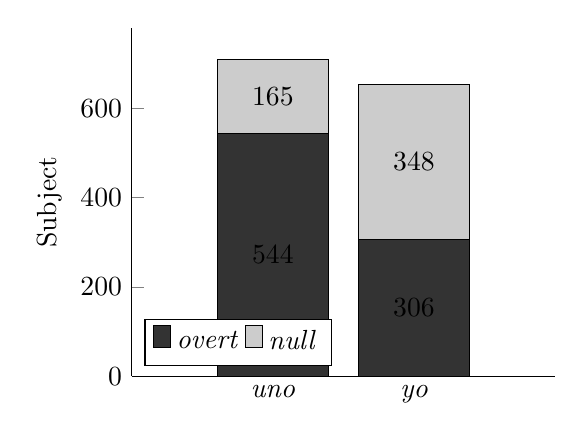
\begin{tikzpicture}
      \begin{axis}
		  [ybar stacked,
           ymin=0,
           ylabel={Subject},
		   bar width=4em,
		   xtick=data,
		   axis lines*=left,
		   symbolic x coords={uno,yo},
		   x tick label style={font=\itshape},
		   nodes near coords,
		   height=6cm,
		   legend pos=south west,
		   legend columns=-1,
		   legend cell align=left,
		   enlarge x limits=1
		  ]
          \addplot+ [black,fill=black!80] coordinates {(uno,544) (yo,306)};
	  	  \addlegendentry{\textit{overt}}
          \addplot+ [black,fill=black!20] coordinates {(uno,165) (yo,348)};
		  \addlegendentry{\textit{null}}
		\end{axis}
  \end{tikzpicture}
  \caption{\label{fig:orozco:1}Distribution of \textit{uno} and \textit{yo} in Medellín}
\end{figure}

\begin{table}
\begin{tabular}{lccr}
\lsptoprule
{Subject type} & \multicolumn{2}{c}{{Variant}} & {Total}\\\cmidrule(lr){2-3}
& {\itshape {uno}}& {\itshape {yo}} & \\
\midrule
Null subjects &  165 (23\%) &  348 (53\%) &  513 (38\%)\\
Overt subjects &  544 (77\%) &  306 (47\%) &  850 (62\%)\\
Total  &  709 (52\%) &  654 (48\%) &  1363 (100\%)\\
\lspbottomrule
\end{tabular}
\caption{Distribution of \textit{uno} and \textit{yo} in Medellín\label{tab:orozco:2}}
\end{table}

Despite \textit{uno} and \textit{yo} being similarly distributed in contexts where they are interchangeable, overt subjects are more frequent with \textit{uno} (77\%) than with \textit{yo} (47\%). That is, they register significantly different overt/null pronominal subject ratios ($\chi^2 = 128.6,\allowbreak p < 0.001$). The much more frequent occurrence of overt subjects with \textit{uno} may stem from the fact that when \textit{uno} occurs in speech, its first occurrence contains an overt subject whereas that is not the case with \textit{yo}. These results, as well as those from Barranquilla, Colombia (\citealt[51]{HurtadoOrtega-Santos2019}), are congruent with the first mention of \textit{uno} being obligatorily overt and its subsequent implications for SPE research. 



\subsection{Conditioning effects on the \textit{uno/yo} alternation}\label{sec:orozco:4.2}


The quantitative model likely to best explain the \textit{uno/yo} alternation in our data sample is illustrated in the random forest consisting of \figref{fig:orozco:2}, which is a graphic representation of \tabref{tab:orozco:3}.\footnote{This random forest was established using Language Variation Suite (\citealt{ScrivnerDíaz-Campos2016}). A random forest is a technique embodied in R that helps determine from a set of predictors those most likely to significantly condition a dependent variable \citep[152]{Tagliamonte2012}, in our case the \textit{uno/yo} alternation. A random forest contributes to enhance the explanatory power of a multivariate regression analysis by providing a visual representation of the conditioning on a given linguistic variable that illustrates the relative importance of each predictor.}   


\begin{figure}
\includegraphics[width=\textwidth]{figures/orozco-2.png}
\caption{\label{fig:orozco:2}Random forest illustrating the analytical model on the variable \textit{uno/yo} alternation in Medellín}
\end{figure}

\begin{table}
\begin{tabular}{lrc}
\lsptoprule
Predictor & \multicolumn{1}{c}{$p$} & { Range}\\
\midrule
Tense, mood \& aspect (TMA) &  $<0.001$ &  77\\
Transitivity &  $<0.001$ &  51\\
Discourse genre  &  $<0.001$ &  34\\
Type of preceding subject  &  $0.003$ &  13\\
Polarity  &  $0.033$ &  10\\
Log likelihood = $-739.9$ & \multicolumn{2}{c}{$\text{AIC}=1517.8$}\\
\lspbottomrule
\end{tabular}
\caption{Analytical model on the variable alternation between \textit{uno} and \textit{yo} in Medellín}
\label{tab:orozco:3}
\end{table}

The quantitative multivariate model of our data sample reveals that the \textit{uno/yo} alternation is significantly conditioned by all five predictors probed in our analysis: TMA, transitivity, discourse genre, type of preceding subject, and polarity. As previously stated (\sectref{sec:orozco:3.4}), this model also includes speaker as well as attenuation procedure and genericity inducers, both tested as a random-effects factors; that is, they were not tested for statistical significance. TMA emerges as the strongest predictor variable, appearing as the farthest from the broken line in \figref{fig:orozco:2} and the predictor with the largest range value (77) in \tabref{tab:orozco:3}. The variation under analysis is also strongly conditioned by transitivity and discourse genre. The difference in the relative conditioning strength of the stronger predictors (TMA, transitivity, and discourse genre) and the weaker ones (type of preceding subject and polarity) is illustrated by the gap that appears in the middle of \figref{fig:orozco:2}, which is also appreciable in \tabref{tab:orozco:3} by the larger range values and smaller but more statistically significant $p$-values for the top three predictors. 



Overall, the conditioning effects on the \textit{uno/yo} alternation validate its status as a legitimate linguistic variable. The results corresponding to the conditioning effects for the different predictors are presented in the following paragraphs according to their statistical ranges and $p$-values; that is, in the same order in which they appear in \tabref{tab:orozco:3}.


\subsection{Verb tense, mood and aspect (TMA)}\label{sec:orozco:4.3}

TMA has the greatest conditioning effect on the \textit{uno/yo} alternation. The results in \tabref{tab:orozco:4} reflect that there are specific contexts of use for either \textit{uno} or \textit{yo}. Infinitives and gerunds – the non-personal verb forms – strongly favor the occurrence of \textit{uno} (0.92). Verbs in the subjunctive mood (0.59) and those in the present indicative – the most frequent tense with 64\% of the data – (0.53) also favor the use of \textit{uno.} At the same time, the imperfect indicative has a neutral effect (0.50) which contrasts with its strongest effect on the alternation between overt and null subjects in this speech community (\citealt{OrozcoHurtado2021}). Conversely, the compound tenses, the conditional and the future – amalgamated as a single factor – (0.25) as well as the preterit indicative (0.15) strongly favor the use of \textit{yo} while disfavoring \textit{uno}. 


\begin{table}
\robustify\bfseries
\begin{tabular}{l S[table-format=1.2] S[table-format=-1.2] S[table-format=2.1] c S[table-format=2.1]}
\lsptoprule
{{Factor}} & {Prob.} & {Log-odds} & {\% \textit{uno}} & {$N$} & {\% data}\\
\midrule
Infinitives \& gerunds                                & \bfseries 0.92 & 2.42  & 91.2 & 52/57   &  4.2\\
Subjunctive                                           & \bfseries 0.59 & 0.35  & 63.9 & 46/72   &  5.3\\
Present Indicative                                    & 0.53          & 0.09  & 55.4 & 486/878 & 64.4\\
Imperfect Indicative                                  & 0.50          & -0.02 & 46.3 & 76/164  & 12.0\\
Other\footnote{Compound tenses, conditional \& future} & 0.25          & -1.12 & 31.6 & 36/114  &  8.4\\
Preterit Indicative                                   & 0.15          & -1.72 & 16.7 & 13/78   &  5.7\\
\multicolumn{1}{r}{{Range = 77}} & \multicolumn{4}{c}{$p<0.001$} &\\
\lspbottomrule
\end{tabular}
\caption{Logistic regression analysis of the effect of TMA on the choice of \textit{uno} in Medellín\label{tab:orozco:4}}
\end{table}

\begin{sloppypar}
These tendencies differ from those registered for SPE in this community (\citealt{OrozcoHurtado2021}). Inter alia, in this analysis we include non-personal verb forms, which are outside the envelope of variation in analyses of the alternation between null and overt pronominal subjects. 
\end{sloppypar}

The conditional inference tree\footnote{This conditional inference tree was established using Language Variation Suite (\citealt{ScrivnerDíaz-Campos2016}). A conditional inference tree, like a random forest, is another technique embodied in R which also contributes to enhance the explanatory power of a multivariate regression analysis by highlighting complex interactions within a dataset. One advantage of a conditional inference tree is that it shows “the subtle interactions in the data using a hierarchical display” \citep[153]{Tagliamonte2012}.}  (\figref{fig:orozco:3}) isolates TMA and transitivity – the two strongest conditioners of the \textit{uno/yo} alternation – from all other predictors. It corroborates that TMA has the greatest conditioning effect on our linguistic variable and transitivity also has a strong effect. Moreover, the conditional inference tree shows how TMA intersects with transitivity. On the left-hand side, node 2 bifurcates into node 4, which contains the TMA factors favoring the occurrence of \textit{uno} (infinitives/gerund and subjunctives), and node 3 which contains the transitivity factors that disfavor \textit{uno} (epistemic clauses). On the right-hand side, node 7 bifurcates into the two TMA factors (preterit indicative and others) that favor \textit{yo} by disfavoring the occurrence of \textit{uno}; that is, nodes 8 and 9, respectively. 

\begin{figure}[H]
\includegraphics[width=\textwidth]{figures/orozco-3.png}
\caption{\label{fig:orozco:3}Conditional inference tree for TMA and transitivity}
\end{figure}

\subsection{Transitivity}\label{sec:orozco:4.4}

The results for transitivity (\tabref{tab:orozco:5}, page \pageref{tab:orozco:5}) uncover that verbs with different degrees of transitivity favor the occurrence of \textit{uno}, regardless of whether \textit{uno} competes with the object for the focus of attention. Instead, epistemic/evidential clauses with one participant promote the occurrence of \textit{yo.} This is an important finding, as it corroborates what previous studies had already indicated: cognitive verbs behave differently with regard to the use of \textit{yo.} In \textit{pronombrista} studies, cognitive verbs have been found to favor first person singular overt pronominal subjects, possibly because the structure of \textit{yo} + epistemic/evidential verbs + clause is so frequent, that it can be considered a “prefabricated unit” (\citealt{TravisTorresCacoullos2012}: 739).


\subsection{Discourse genre}\label{sec:orozco:4.5}

As \tabref{tab:orozco:6} (page \pageref{tab:orozco:6}) shows, opinion statements strongly promote \textit{uno} with a statistical weight of 0.71. At the same time, hypothetical situations exert a neutral effect (0.47) whereas narrations favor the selection of \textit{yo.} These findings clearly indicate that the link between \textit{yo} and the most personal discursive types, on the one hand, and \textit{uno} with argumentative discourse, on the other, is maintained. Because narrations mainly consisted of reporting events that happened in the past or were currently happening at data collection time, those actions are considered realis forms, high in transitivity (\citealt{HopperThompson1980}). As irrealis forms are low in transitivity, attention is focused on the subject, in this case, expressed by \textit{uno}. This use could be explained as a mitigation strategy, as the speaker expresses opinions. 


\begin{table}[p]
\begin{tabularx}{\textwidth}{Q c S[table-format=1.2] S[table-format=-1.2] S[table-format=2.1] c S[table-format=2.1]}
\lsptoprule
{Factor} & \#P & {Prob.} & {Logodds} & {\% \textit{uno}} & {$N$} & {\% data}\\
\midrule
Verb with prepositional complement & 2 &  0.67 &  0.71 &  64.4 &  29/45 &  3.3\\
Intransitive & 1 &  0.59 &  0.35 &  56.7 &  216/381 &  28.0\\
Transitive & 2/3 &  0.59 &  0.38 &  56.0 &  255/455 &  33.4\\
Reflexive & 1 &  0.56  &  0.25 &  55.0 &  116/211 &  15.5\\
Transitive with null object & 2&  0.50 &  0.01 &  44.9 &  53/118 &  8.7\\
Epistemic + complement clause &1&  0.16 &  -1.70 &  26.1 &  40/153 &  11.2\\
\multicolumn{2}{c}{{  Range = 51}} & \multicolumn{3}{c}{$p <0.001$} & \\
\lspbottomrule
\end{tabularx}
\caption{Logistic regression analysis. Effect of transitivity and competition for the focus of attention on the use of \textit{uno} in Medellín. “\#P”: Number of participants}
\label{tab:orozco:5}
\end{table}

\begin{table}[p]
\begin{tabularx}{\textwidth}{Q S[table-format=1.2] S[table-format=-1.2] S[table-format=2.1] c S[table-format=2.1]}

\lsptoprule
{Factor} & {Prob.} & {Logodds} & {\% \textit{uno}} & {$N$} & {\% data}\\
\midrule
Opinion & \bfseries .71 & 0.89 & 68.9 & 354/514 & 37.7\\
Hypothetical situations  & .47 & -0.12 & 49.7 & 99/199 & 14.6\\
Narrative & .32 & -0.77 & 39.4 & 256/650 & 47.7\\
\multicolumn{2}{c}{{Range = 37}} & \multicolumn{3}{l}{$p <0.001$} &\\
\lspbottomrule
\end{tabularx}
\caption{Logistic regression analysis. Effect of discourse genre on the choice of \textit{uno} in Medellín}
\label{tab:orozco:6}
\end{table}

\begin{table}[p]
\begin{tabularx}{\textwidth}{Q S[table-format=1.2] S[table-format=-1.2] S[table-format=2.1] c S[table-format=2.1]}
\lsptoprule
\multicolumn{1}{c}{Factor}&{Prob.}&{Logodds}&{\%\textit{uno}}&{$N$}&{\%data}\\
\midrule
Overt subjects   & .56 & 0.22 & 57.6 & 285/495 & 36.3\\
Others          &.52 & 0.07 & 53.9 & 173/321 & 23.6\\
Null subjects   & .43 & -0.29 & 45.9&251/547&40.1\\
\multicolumn{2}{c}{{Range = 13}}& &\multicolumn{2}{c}{$p=0.003$}&\\
\lspbottomrule
\end{tabularx}
\caption{Logistic regression analysis. Effect of type of preceding subject on the choice of \textit{uno} in Medellín}
\label{tab:orozco:7}
\end{table}

\subsection{Type of preceding subject}\label{sec:orozco:4.6}



As \tabref{tab:orozco:7} (page \pageref{tab:orozco:7}) shows, preceding overt pronominal subjects favor the selection of \textit{uno} with a statistical weight of 0.56, confirming that an overt pronoun precedes a coreferent \textit{uno}. Preceding null subjects, by disfavoring \textit{uno}, promote the occurrence of \textit{yo} (0.43). Concurrently, all other subjects (lexical subjects and demonstratives) have a neutral effect (0.52).

The conditioning effect of type of preceding subject is similar to what happens across the board with SPE (\citealt{CameronFlores-Ferrán2004}), which has been attested in several Colombian speech communities including Medellín (\citealt{OrozcoHurtado2021}), Cali (\citealt{TorresCacoullosTravis2019}), Barranquilla, and the New York City Colombian enclave \citep[104]{Orozco2018}, respectively. Moreover, these tendencies uncover that the conditioning effect of priming on variation in Spanish extends to the \textit{uno/yo} alternation.   

\subsection{Polarity}\label{sec:orozco:4.7}



Results for polarity (\tabref{tab:orozco:8}) reveal that affirmative statements favor the occurrence of \textit{uno} with a probability weight of 0.55. Nevertheless, negative statements favor the occurrence of \textit{yo} with a weight of 0.45, a tendency contrary to findings by \citet{Flores-Ferrán2009}. 


\begin{table}
\begin{tabular}{l S[table-format=1.2] S[table-format=-1.2] S[table-format=2.1] c S[table-format=2.1]}
\lsptoprule
\multicolumn{1}{c}{Factor} & {Prob.} & {Log-odds} & {\% \textit{uno}} & {$N$} & {\% data}\\
\midrule
Affirmative &  .55 &  0.22 &  54.1 &  629/1162 &  85.3\\
Negative &  .45 &  -0.22 &  39.8 &  80/201 &  14.7\\
\multicolumn{3}{c}{{Range = 10}} & \multicolumn{2}{c}{$p = 0.033$} &\\
\lspbottomrule
\end{tabular}
\caption{Logistic regression analysis. Effect of polarity on the choice of \textit{uno} in Medellín\label{tab:orozco:8}}
\end{table}

\subsection{Attenuation procedure and genericity inducers}\label{sec:orozco:4.8}


The effects of the attenuating procedure on the \textit{uno/yo} alternation reveal the pragmatic dynamics involved in the expression of impersonality. Due to the nature of this predictor,\footnote{Attenuation procedure and genericity inducers comprise what for a multivariate regression constitutes a large number of factors – initially 18; later reduced to 14 – which would render skewed results if included in a multivariate analysis.}  as indicated above (\sectref{sec:orozco:3.4}), we tested its effect as a random effects factor to measure the pragmatic conditioning on the alternation between \textit{uno} and \textit{yo}. In general (see \tabref{tab:orozco:9}), we found that \textit{uno} favors the use of attenuating elements more than \textit{yo,} which suggests that the greater the number of resources available to the speaker, the higher the degree of mitigation \citep[368]{CesteroMancera2020}. The speaker uses \textit{uno} as follows:


\begin{itemize}
\item to reduce their agentivity by placing the subject in a postverbal position (0.75);  
\item with two or three more attenuating elements (0.65);
\item in justifying or apologizing constructions (0.64);
\item with adverbial inductors of genericity – especially adverbs of time – (0.57); 
\item with resources that involve the addressee to draw the interlocutor’s attention (0.54); and 
\item with diminutives (0.53). 
\end{itemize}

Conversely, \textit{yo} is used mainly without attenuating elements, with strategies expressing doubt, probability and reformulation, with resources that impersonalize, and especially with epistemic markers that indicate uncertainty, lack of knowledge or competence (34 of 39 cases), such as \textit{no sé} ‘I don’t know’ to establish their personal deixis \citep{Caffi2007}. 

\begin{sidewaystable}
\begin{tabular}{>{\raggedright}p{9cm} S[table-format=1.2] S[table-format=-1.2] S[table-format=2.1] c S[table-format=2.1]}
\lsptoprule
\multicolumn{1}{c}{Factors} & {Prob.} & {Intercept} & {\% \textit{uno}} & {N} & {\% data}\\
\midrule
Postverbal subject  & \bfseries .75 & 1.10 & 80.4 & 82/102 & 7.5\\
2 or 3 attenuating elements & \bfseries .65 & 0.59 & 62.8 & 27/43 & 3.2\\
Resources that justify  & \bfseries .64 & 0.56 & 66.1 & 72/109 & 8.0\\
Adverbs of time, place and mood & \bfseries .57 & 0.27 & 66.0 & 33/50 & 3.7\\
Resources that involve the addressee & .54 & 0.14 & 50.0 & 13/26 & 1.9\\
Diminutive suffixes & \bfseries .53 & 0.12 & 58.3 & 14/24 & 1.8\\
Approximators or diffusers of meaning & .49 & -0.06 & 57.0 & 61/107 & 7.9\\
Objectivization using modal discourse particles& .49 & -0.05 & 50.0 & 9/18 & 1.3\\
Resources that limit or restrict\footnote{(concessivity, expressions with conditional meaning, modal use of verb tenses)}  & .47 & -0.11 & 48.1 & 37/77 & 5.6\\
Verbs and particles that express doubt or probability& .45 & -0.19 & 40.6 & 13/32 & 2.3\\
Resources that correct or reformulate & .44 & -0.26 & 44.7 & 21/47 & 3.4\\
Absence of attenuating elements & .42 & -0.31 & 46.7 & 314/673 & 49.4\\
Resources that impersonalize & .38 & -0.50 & 50.0 & 8/16 & 1.2\\
Verbs and particles that feign uncertainty, incompetence or ignorance & .20 & -1.37 & 12.8 & 5/39 & 2.9\\
\lspbottomrule
\end{tabular}
\caption{Effects of attenuation procedure and genericity inducers on \textit{uno} in Medellín}
\label{tab:orozco:9}
\end{sidewaystable}

In previous SPE investigations (cf. \citealt{Flores-Ferrán2009}), \textit{uno} has been analyzed in terms of its morphosyntactic properties. This investigation extends the analytical scope to its pragmatic properties. 


\section{Discussion}\label{sec:orozco:5}


This variationist investigation has explored the alternation between the Spanish subject pronouns \textit{uno} and \textit{yo} – an underexplored pronominal expression phenomenon – in terms of the extension of \textit{uno} to other morphosyntactic and semantic domains, mainly that of first person singular. Our study has addressed three research questions and a main hypothesis. Interestingly, \textit{uno} and \textit{yo} are interchangeable when they occur within a single speech turn even if they do not indicate impersonality. In fact, in our data sample, they are interchangeable in 1363 or 82\% of the 1582 clauses with either pronoun as the subject. The answer to our first research question (\textit{How are} uno \textit{and} yo \textit{distributed when they appear interchangeably within a single speech turn, and what predictor variables condition their alternation?}) reveals that both pronouns are similarly distributed although \textit{uno} (52\%) is slightly more frequent than \textit{yo} (48\%). The internal predictors that most strongly condition the \textit{uno}/\textit{yo} alternation are TMA, transitivity, and discourse genre. Our analysis uncovered that \textit{uno} is favored by low transitivity contexts such as impersonal verb forms (infinitives and gerunds), imperfective actions (present indicative) and irrealis forms (subjunctive mood and opinion), which promote the focus of attention to remain on the subject. Concurrently, \textit{yo} is favored in high transitivity contexts where the focus is more on the action and the object, as happens in perfective actions (preterit) and realis discursive types such as narration. 



The findings for TMA are especially important, not only because this predictor exerted the strongest conditioning influence, but also because they partially support the premise that actions involving impersonal pronouns are framed preferentially in the habitual present and the imperfect (\citealt{MuñizCachón1998}), given that the imperfect indicative has a neutral effect, as example \REF{ex:orozco:12} illustrates.  


\eanoraggedright\label{ex:orozco:12}
\begin{xlist}[‘E:]
\exi{{E.:}}{¿y qué le dijo su familia de eso?}
\exi{‘E:}{And what did your family tell you about that?}
\exi{{I.:}} {{no las niñas hermano / fue que la señora es la que me vio cuando} \ExHighlight{{[∅]} \ExHighlight{subí}} {sin zapatos // no lo que pasó /} \ExHighlight{{yo} \ExHighlight{cuando} \ExHighlight{subí} \ExHighlight{/} \ExHighlight{yo} \ExHighlight{me} \ExHighlight{acuerdo}} {que} \ExHighlight{{[∅]} \ExHighlight{subí}} {la subida y} \ExHighlight{{[∅]} \ExHighlight{no} \ExHighlight{me} \ExHighlight{acuerdo}} {quién había y quién no …} \ExHighlight{uno} / \ExHighlight{uno} \ExHighlight{se} \ExHighlight{achanta} {y / todas esas veces que} \ExHighlight{{se} \ExHighlight{toma} \ExHighlight{uno}} {unas cervecitas por ahí en el centro /} \ExHighlight{{yo} \ExHighlight{me} \ExHighlight{alejé}} {/ pues} \ExHighlight{{[∅]} \ExHighlight{me} \ExHighlight{he} \ExHighlight{alejado}} {de todo eso.} (MEDE H11{}-2)}
\exi{`I.:}\glt  no, the girls brother / my wife was the one who saw me when [\ExHighlight{I}] \ExHighlight{went}\textsubscript{1} upstairs shoeless // no, what happened / when \ExHighlight{I} \ExHighlight{went}\textsubscript{2} upstairs / \ExHighlight{I} \ExHighlight{remember}\textsubscript{3} that [\ExHighlight{I}] \ExHighlight{went}\textsubscript{4} upstairs and [\ExHighlight{I}] \ExHighlight{don't} \ExHighlight{remember}\textsubscript{5} who was there and who wasn’t ... \ExHighlight{one} / \ExHighlight{one} \ExHighlight{backs} \ExHighlight{down}\textsubscript{6} and / all those times when \ExHighlight{one} \ExHighlight{drinks}\textsubscript{7} a few beers around downtown / \ExHighlight{I} \ExHighlight{backed}\textsubscript{8} away/ well [\ExHighlight{I}] \ExHighlight{have} \ExHighlight{backed}\textsubscript{9} away from all that.’ 
\end{xlist}
\z 

The strongest favoring effect of non-finite forms (infinitives and gerunds amalgamated as a single factor [0.92]) on \textit{uno} can be related to the premise that, as these forms do not provide morphological information about tense, aspect and person, they are often used as infinitives of generic interpretation (\citealt{NuevaGramática2009}: 2002). Our results also concur with those of \citegen{Flores-Ferrán2009}, given that \textit{uno} was also used more frequently in preposition + subject + infinitive constructions (39\%). There were also cases in which the infinitive appears after subordinate clauses (14.6\%), with the occurrence of \textit{uno} + infinitive subordinated to a subjunctive clause, as example \REF{ex:orozco:13} illustrates. This also occurs frequently in our data in the coreference between subjects with infinitives and the subject of the subordinating clause whose verb occurs in the subjunctive \REF{ex:orozco:14}:

\eanoraggedright\label{ex:orozco:13}
{¿Qué} \ExHighlight{{[∅]} \ExHighlight{pienso?}} {pues / ojalá que cambie / ojalá que cambie / porque} \ExHighlight{{uno} \ExHighlight{ver} \ExHighlight{uno} }{por donde pasa y //} \ExHighlight{{[∅]} \ExHighlight{ve}} {gente muerta y // eso es muy duro} \ExHighlight{{uno} \ExHighlight{ver}} {gente ahí tirada.} (\ExHighlight{MEDE\_} \ExHighlight{M11\_4)}
\glt {‘What} \ExHighlight{{do} \ExHighlight{I} \ExHighlight{think}}{? well [I hope] it changes/ hopefully [it] will change because} \ExHighlight{{one} \ExHighlight{to} \ExHighlight{see} }{where} \ExHighlight{{one} \ExHighlight{passes}} {and [}\ExHighlight{{one}}] \ExHighlight{{sees}} {dead people and // that is very hard} \ExHighlight{{one} \ExHighlight{to} \ExHighlight{see}} {people lying there.’}
\ex\label{ex:orozco:14}
\begin{xlist}[`E.:]
\exi{{E.:}}{{¿qué es lo que más le gusta? / algún espacio / ¿o le gusta porque se siente cómodo? / ¿qué es lo que más le gusta de su casa?}}
\exi{`E.:}{‘What do you like best? / some space / or do you like it because you feel comfortable? / what do you like most about your house?’}
\exi{{I.:}}{{Pues que} \ExHighlight{{uno} \ExHighlight{se} \ExHighlight{sienta}} {cómodo /} \ExHighlight{{estar}} {bien esto y esto}. (\ExHighlight{MEDE\_H11\_2)}}
\exi{`I.:}{‘Well that} \ExHighlight{{one} \ExHighlight{feels}} {comfortable /} \ExHighlight{{to} \ExHighlight{be}} well this and this.’
\end{xlist}
\z 


In both cases, the infinitive obtains temporal information from the predicates to which it is subordinated (\citealt{NuevaGramática2009}: 1976).



However, when we analyzed the role of the number of participants, we found no effect of the competition for the focus of attention on the selection of \textit{uno}. Instead, \textit{yo} was considerably favored by epistemic/evidential verbs that introduce complement clauses, in which the speaker expresses a stance toward the content of that clause. This is an important finding because \citet{Posio2011} and \citet{HurtadoOrtega-Santos2019} have found a correlation between low transitivity verbs with one participant and the overt expression of \textit{yo} and \textit{uno}, respectively. Our findings regarding the \textit{uno/yo} alternation corroborate that besides the influence of low transitivity verbs and the focus of attention on the subject, speakers also favor \textit{yo} to express a stance with epistemic verbs, as suggested by \citet{Posio2011}. The use of \textit{yo} with low transitivity verbs is also evident in the favoring effect of the attenuation procedure of expressing uncertainty, incompetence or ignorance. \textit{No sé} ‘I don’t know’ was the recurrent form in this category, a negated verb which indicates the degree of commitment of the speaker toward what is said. It is also interesting that, in Medellín, the use of \textit{yo} happens not only with this downgrading strategy that involves the speaker, but also with impersonalization mechanisms that indicate distancing from the speaker \citep{CesteroMancera2020}. 



The answer to our second research question (\textit{In what discursive contexts are} uno \textit{and} yo \textit{used interchangeably?}) reveals that, in certain interchangeable contexts, \textit{uno} and \textit{yo} share the same tendencies: with present indicative and hypothetical situations; with attenuation procedures that limit or restrict (concessivity, expressions with conditional meaning, modal use of verb tenses), modal discourse particles for objectivization, and approximators. These findings contribute to validate the premise that \textit{uno} has extended semantically and pragmatically beyond the third person singular – as it is morphosyntactically inflected – to contexts now shared with the first-person singular pronoun.  



The tendencies for discourse genre contribute to answer our third research question (\textit{What functions are most commonly assumed by each pronoun, and how do} uno \textit{and} yo \textit{construct/create the discursive subject?}), as they suggest a clear differentiation of discursive functions. \textit{Uno} assumes the function of expressing opinions about the city and its people, whereas \textit{yo} assumes narrative functions (personal experiences). Concomitantly, both pronouns equally facilitate the formulation of hypothetical discourse. Despite the tendencies for the other predictors that condition the \textit{uno/yo} alternation not reflecting a clear differentiation of functions, \textit{uno} appears to facilitate the expression of the subjunctive and non-personal verb forms, overt pronominal subjects, and postverbal subjects, respectively. On the other hand, \textit{yo} appears to assume the expression of the preterit, epistemicity, null subjects, as well as that of verbs and particles that feign uncertainty, incompetence, or ignorance.   



With regard to TMA, the strongest favoring effect of impersonal forms on \textit{uno} (statistical weight 0.92) highlights the effect of a factor that is not measured in classic \textit{pronombrista} studies because non-finite, impersonal forms are outside the SPE envelope of variation given that such forms do not facilitate the identification of the grammatical person of a null subject (\citealt{OtheguyZentella2012, Orozco2018}). Concurrently, a priming effect is evident, as the tendencies for type of preceding subject uncover the favorable effect of a preceding overt subject on \textit{uno} whereas \textit{yo} is promoted by preceding null subjects. This priming effect, being similar to the priming effect on SPE, constitutes a structural commonality between the \textit{uno/yo} alternation and the alternation between null and overt pronominal subjects.   



\section{Conclusion}\label{sec:orozco:6}


The present variationist study corroborates the strong effect of \textit{uno} promoting the occurrence of overt pronominal subjects previously reported in Medellín (\citealt[717]{OrozcoHurtado2021b}). Here we have shown how \textit{uno} has entered the morphosyntactic and semantic domain of the first person singular. Our results uncover that there is not a complete reduction of the impersonal reference in all cases where \textit{uno} and \textit{yo} alternate as sentential subjects within a single speech turn. Among other things, our analysis has demonstrated that the \textit{uno/yo} alternation constitutes a linguistic variable in its own right. Along with the goals of this volume, this chapter contributes to augment our collective knowledge of pronominal expression and related linguistic phenomena. Our investigation also contributes to show that the analysis of pronominal expression still has much to contribute to the study of language variation and change.  

\printbibliography[heading=subbibliography]

\end{document}
